%!TEX root = ../thesis.tex

\chapter{Method}
\label{ch:method}


\section{Energy simulations}
\subsection{Production}
Since this project cannot gather data of production from the systems, a simulation is useful for creating an estimation of this. In this case, we have specifications of equipment and location to test out. The systems are delivered from Bright, and are three different sizes. The three systems are given in table \ref{table:product_specifications}. 

\begin{table}[h]
\centering
\begin{tabularx}{\textwidth}{|X|X|X|X|}
\hline
\textbf{Product name} & \textbf{Battery capacity [Wh]} & \textbf{Panel size [Wp]} & \textbf{Total lumen} \\ \hline
BH 300                &            29                    &          10                 &         360               \\ \hline
BH 600                &              58                  &          20                 &           760             \\ \hline
BH 800                &              80                  &         40                  &            1400            \\ \hline
\end{tabularx}
\caption{Product specifications of Bright SHS}
\label{table:product_specifications}
\end{table}

Using this we have three different scenarios we can simulate with. Further we need to locate the weather data to use for this. The \acrfull{pvgis} can be used as a trusted data source to simulate with specific weather data for a location\citep{huldNewSolarRadiation2012}.

Using that we have a 40Wpp PV panel, we can use the PVGIS to simulate the power generation for each month. The PVGIS assumes a 14\% power loss in the transmission. Since we don't have any more accurate data, this will be used in the simulation. Potential soiling will be added as power loss in results. On figure \ref{method:fig:wattage_generation_PV40wpp} we can see how each month differs in the power generated. Each month has been given a mean to account for good or bad days. This will give us a good indication of what a typical day will generate during a day, and when it will generate the power. When we combine this with a daily load profile, we can analyze well the system is utilized. 

\begin{figure}[H]
    \centering
    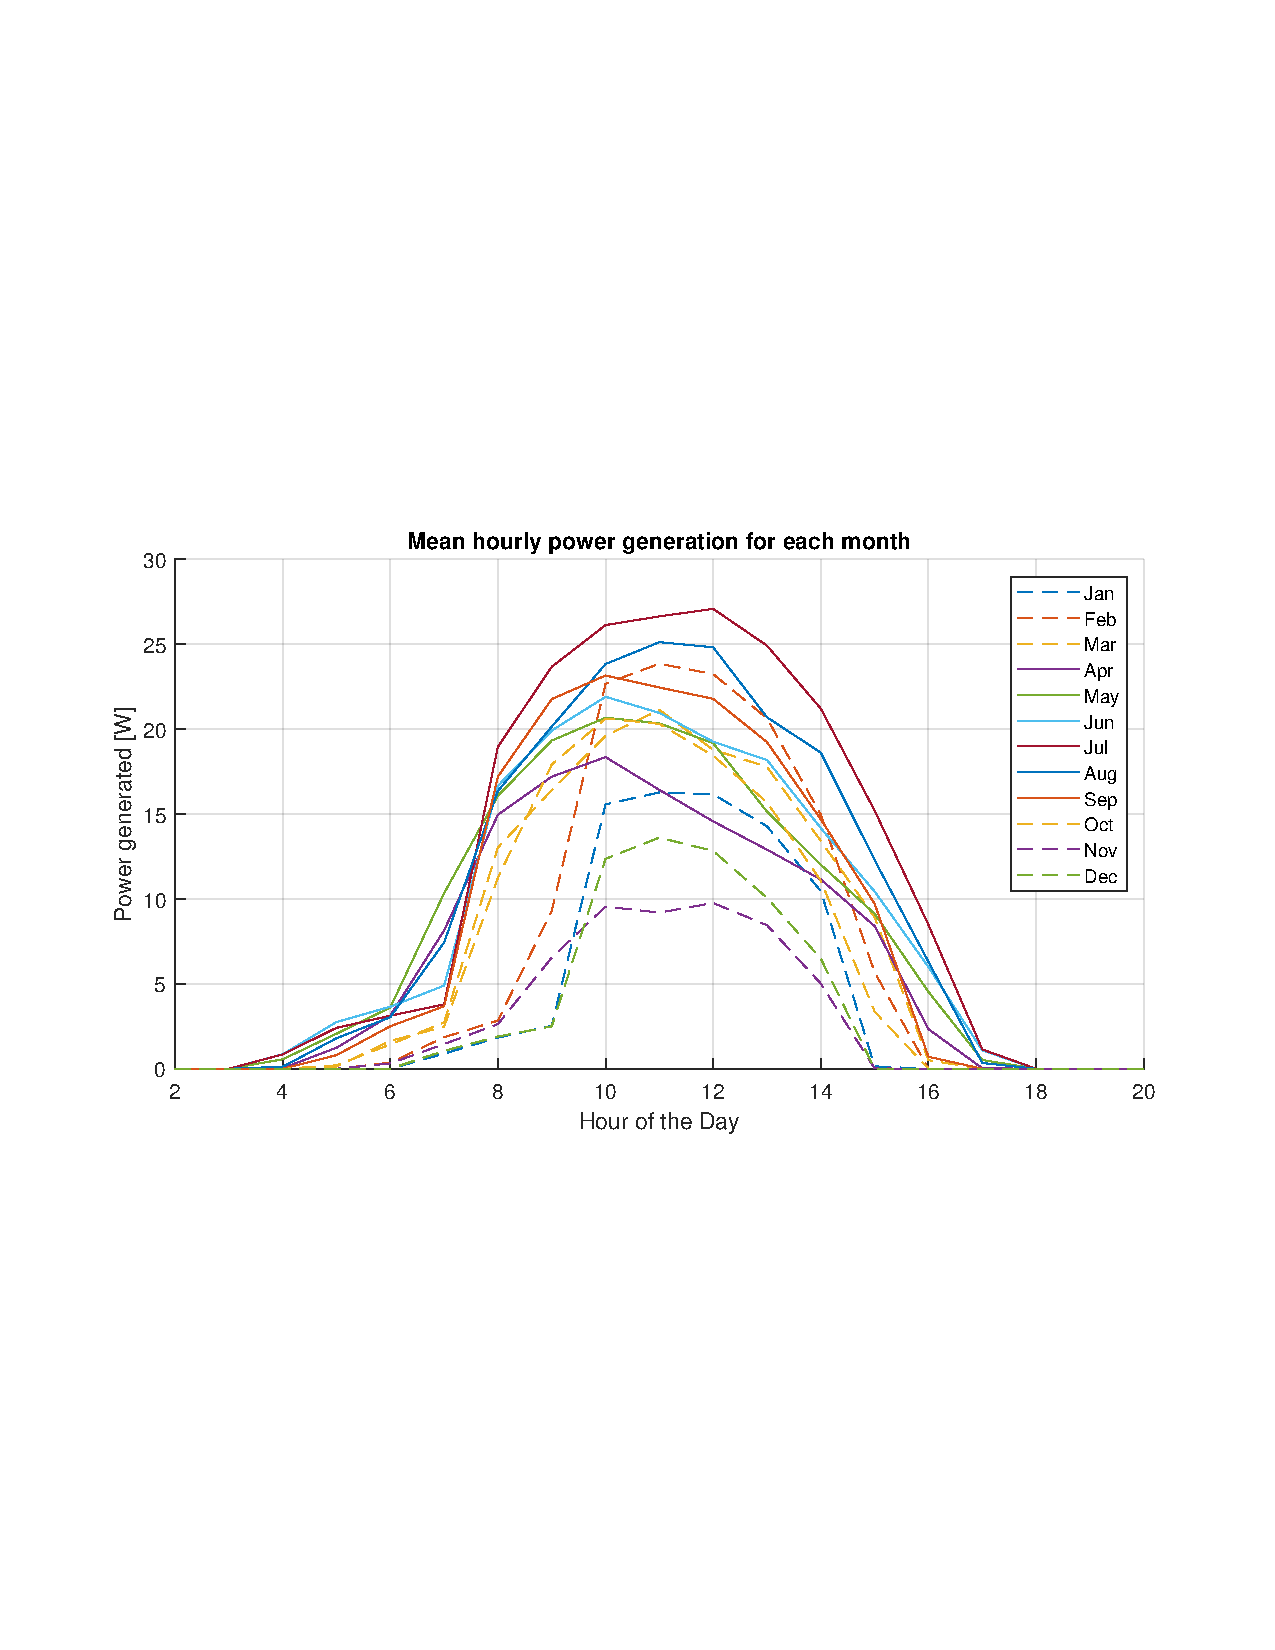
\includegraphics[width=\linewidth]{photos/Watt_generated_Shkoder.pdf}
    \caption{Power generation from a 40Wpp panel in the Shkodër region with tilt angle $\alpha=35\degree$, and azimuth $\phi=23\degree$.}
    \label{method:fig:wattage_generation_PV40wpp}
\end{figure}

The months with the least daylight has been given a dotted line, and the ones with the most have a solid line. From this we can see that the trend of most light in "winter" months is not always true. February and April will be almost equal in this simulation, showing how much factors such as rain, clouds and angle will affect the panel power generation. 

In table \ref{method:table:wattage_generation_per_month_all_panels} we can see how much each is generated for a typical day, here the values confirm what the graph is showing.
\begin{table}[H]
\centering
% For bedre talljustering i X-kolonner kan du vurdere >{\raggedleft\arraybackslash}X,
% eller for optimal talljustering, bruk siunitx-pakken og S-kolonner.
% For enkelhetens skyld beholder vi X-kolonner som i din originale tabell.
\begin{tabularx}{\textwidth}{|X|S[table-format=3.1]|S[table-format=3.1]|S[table-format=3.1]|}
% table-format=3.1 betyr opptil 3 siffer før desimaltegnet, og 1 siffer etter.
\hline
\textbf{Month} & \textbf{40Wpp [Wh]} & \textbf{20Wpp [Wh]} & \textbf{10Wpp [Wh]} \\ \hline
January        & 78.1                & 39.1                & 19.5                \\ \hline
February       & 125.4               & 62.7                & 31.4                \\ \hline
March          & 133.9               & 67.0                & 33.5                \\ \hline
April          & 128.9               & 64.4                & 32.2                \\ \hline
May            & 153.5               & 76.7                & 38.4                \\ \hline
June           & 160.7               & 80.4                & 40.2                \\ \hline
July           & 203.6               & 101.8               & 50.9                \\ \hline
August         & 180.9               & 90.5                & 45.2                \\ \hline
September      & 157.7               & 78.9                & 39.4                \\ \hline
October        & 122.9               & 61.5                & 30.7                \\ \hline
November       & 52.9                & 26.5                & 13.2                \\ \hline
December       & 60.8                & 30.4                & 15.2                \\ \hline
\end{tabularx}
\caption{Estimated daily energy production for 40Wpp, 20Wpp, and 10Wpp panel}
\label{method:table:wattage_generation_per_month_all_panels} % Endret label for unikhet om nødvendig
\end{table}
For all three systems, November, December and January is the only months that the daily production will not exceed the battery capacity. Incomplete charges can over time lead to an empty battery. It could then take several days with minimal use for the system to get fully charged again. 

These production numbers assume optimal angle and azimuth. In results chapter \ref{ch:results}, we look at both the average azimuth and the tilt angle. We will also have to account for other loss factors, such as soiling. Then we can do a more precise estimation of the daily production of the PV panel. 


\subsection{Consumption}
To gather the daily load profile, we will have to ask questions from the participants. Based on their answers we can create a daily load using the known power of having the lights on, or USB-A power delivery. The questions used for this data gathering needs to gather both how much power is used, and when it is used. There will always be some uncertainty around the numbers, and the actual usage will vary from day to day. 

Seasonal variation of the consumption is hard to measure, but can be estimated from the answers given. The difference between the shortest and longest day in Shkodër is about six hours\citep{steffenthorsenSunriseSunsetTimes2025}, meaning the systems production and consumption will vary due to seasonal differences. Longer nights leads to more usage of light from the system. Shorter days reduces the time for the panels to charge the system. Although the production is simple to find accurate data for, the seasonal differences of consumption is harder.

The duck curve is used to describe the dilemma of solar power generation being most useful when least needed\citep{krietemeyerManagingDuckCurve2021}. As PV panels are most effective at midday, and that happens to be when electricity is lowest in demand - resulting in a drop that is called the duck curve. This duck curve is also applicable to the SHS, as their main purpose is to supply lights at night from the charge during the day. 

\citep{sevdariDataDrivenAssessmentElectricity2022} gives a dataset of three years of electricity load we can analyze. In figure \ref{method:fig:gridloadalbania} we see the average hourly load from this dataset.
\begin{figure}[H]
    \centering
    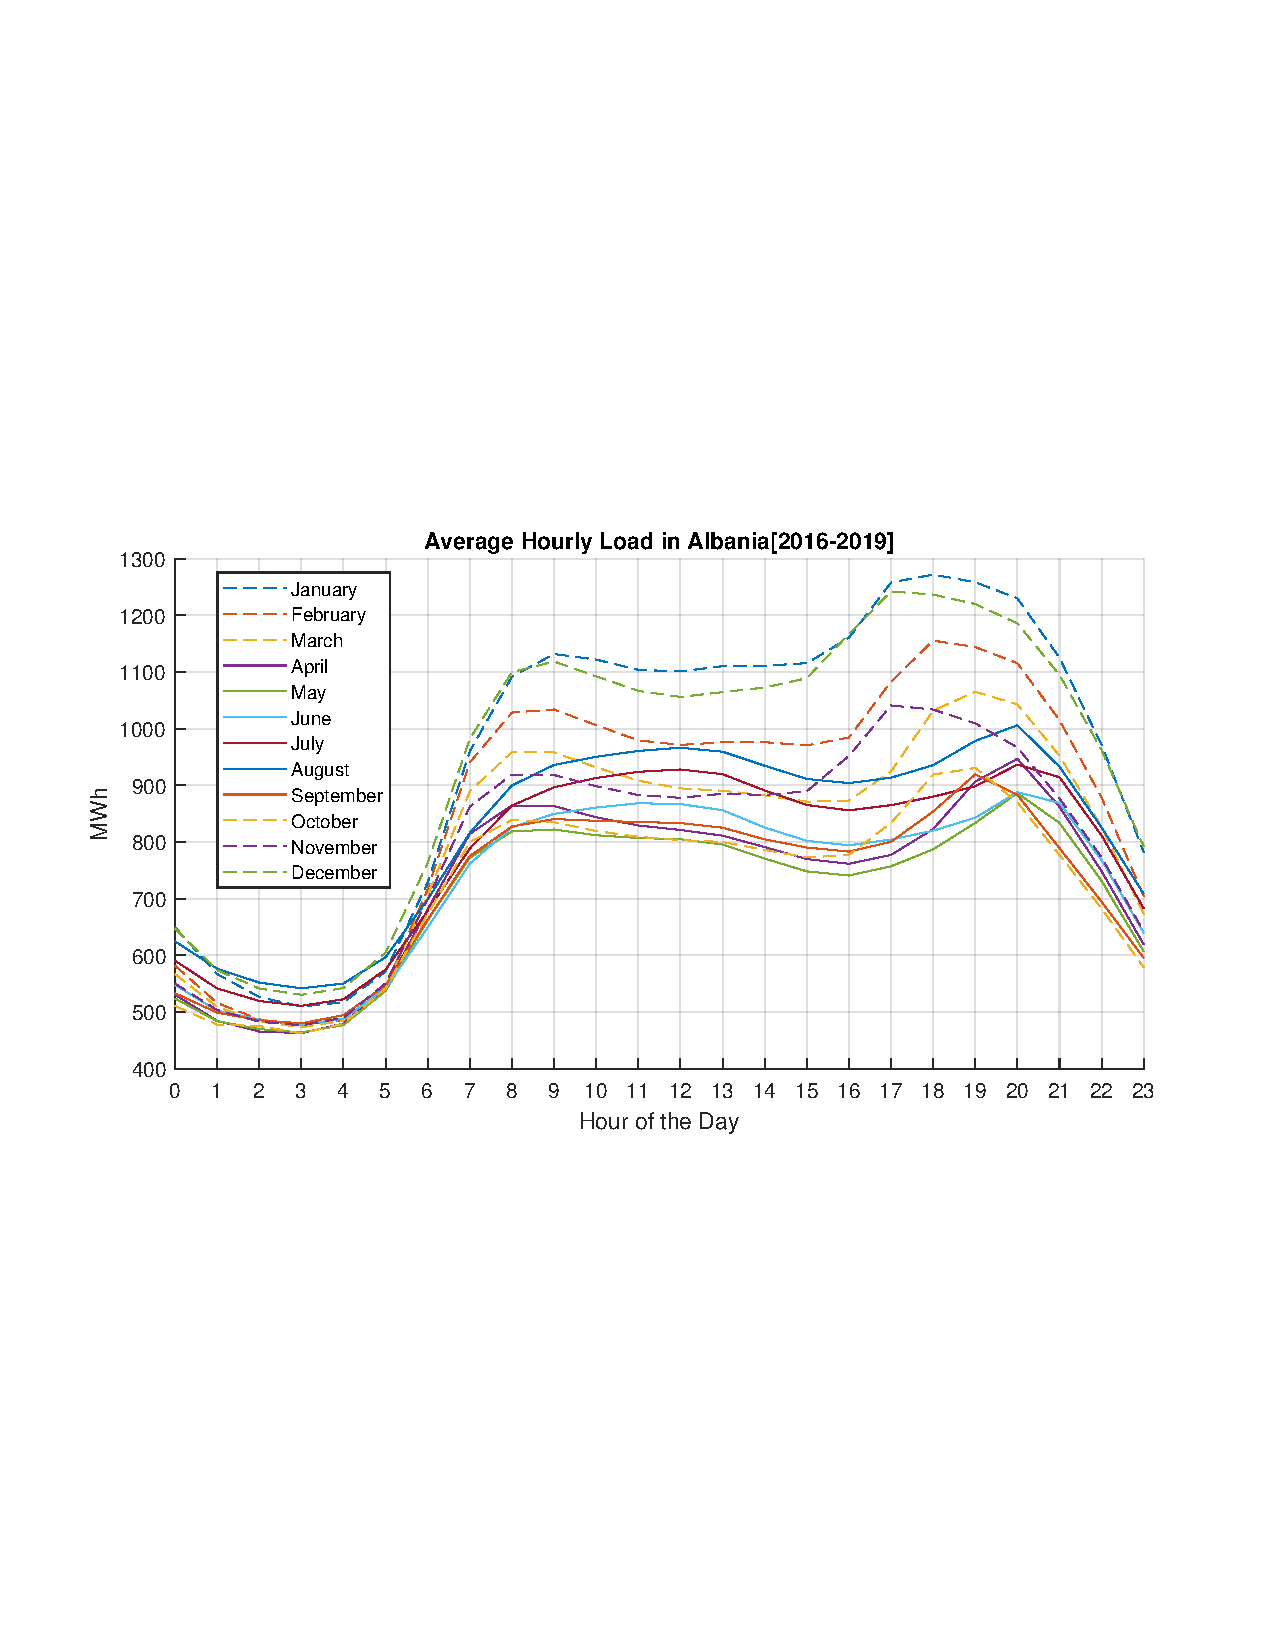
\includegraphics[width=\linewidth]{photos/GridLoadAlbania_2016-2019.pdf}
    \caption{Hourly average of national grid load in Albania from 2016 to 2019. Sorted into average for each month. The winter half-year is dotted to show consumption in these months}
    \label{method:fig:gridloadalbania}
\end{figure}
As mentioned, Albania does not produce much solar power. Meaning this curve will not drop in the midday as the duck curve, and rather flat out. This relationship will change if the household energy mix includes a SHS, as this can produce excess during the day. 

Winter months are consistently higher load than summer months. We can also see a noticeable shift in where the evening peak starts. December and January has their peak at about 17, while summer months peak at 20. The difference is not seen as much in the morning peak. 

\subsection{Daily load profile}
There are three different power settings on the system, and the various systems have different amount of lighting. As mentioned in table \ref{table:product_specifications}, the systems vary from 360 to 1400 lumen based on power setting. The larger system has more light modules that can be connected than the smaller systems. In table \ref{table:light_inventory} we see the inventory of each system. 

%% husk å legg inn hvor lenge de holder i timer for hver setting
\begin{table}[h]
\centering
\begin{tabularx}{\textwidth}{|X|S[table-format=3.1]|S[table-format=3.1]|S[table-format=3.1]|S[table-format=3.1]|S[table-format=3.1]|}
\hline
\textbf{System} & \textbf{Fixed-focus lamps} & \textbf{Tube lights}  &\textbf{USB-A}& \textbf{Min [lm]} & \textbf{Max  [lm]} \\ \hline
BH 300                &               3              &          0    & 2     & 30    & 360 \\ \hline
BH 600                &              3                  &          1   & 2    &   230 & 760 \\ \hline
BH 800                &              3                  &         2    & 2    & 520  & 1400 \\ \hline
\end{tabularx}
\caption{Light module inventory of systems. \textit{Min [lm]} is when all lights on low power setting, \textit{Max [lm]} is when all lights are on full power setting.}
\label{table:light_inventory}
\end{table}

Depending on the power setting and the amount of light, the systems deliver different lumen. Achieving higher lumen at higher power consumption. Table \ref{table:power_configurations_all_systems} shows the consumption for different scenarios in the systems. Power setting, amount of lights and charging via USB all change the power consumption. 

\begin{table}[h!]
\centering
\small % Applied to the whole table float
% Main caption for the entire set of subtables
\caption{Power consumption for BH systems under various operational configurations. Each sub-table details scenarios for a specific system. Systems $S_3, S_6, S_8$ correspond to BH 300, BH 600, and BH 800 and their inventory from Table \ref{table:light_inventory}. Columns \textit{Fixed}, \textit{Tube} and \textit{USB} indicate the number of active components. \textit{Power Setting} shows which power settings the lights are on, $P_L$ (low), $P_M$ (medium), $P_H$ (high). $P_F$, $P_t$ and $P_U$ correspond to the power consumption from \textit{Fixed}, \textit{Tube} and \textit{USB}. $P_{total}$ is the combined power consumption.}
\label{table:power_configurations_all_systems}
\begin{subtable}{\textwidth}
    \centering
    \begin{tabularx}{\linewidth}{|C|S[table-format=1.0]|S[table-format=1.0]|S[table-format=1.0]|C|S[table-format=4.0]|S[table-format=4.0]|S[table-format=5.0]|c|}
    \hline
    \textbf{System} & \textbf{Fixed} & \textbf{Tube} & \textbf{USB} & \textbf{Power Setting} & \textbf{$P_F$ [mW]} & \textbf{$P_T$ [mW]} & \textbf{$P_U$ [mW]} & \textbf{$P_{total}$ [mW]} \\ \hline
    % Data for System S3 (BH 300)
    $S_3$  & 1   & 0   & 0   & $P_L$         & 348        & 0          & 0          & \cellcolor{LightGray}348             \\ \hline
    $S_3$  & 3   & 0   & 0   & $P_H$         & 5760       & 0          & 0          & \cellcolor{LightGray}5760            \\ \hline
    $S_3$  & 2   & 0   & 0   & $P_L$         & 696        & 0          & 0          & \cellcolor{LightGray}696             \\ \hline
    $S_3$  & 3   & 0   & 0   & $P_L$         & 1044       & 0          & 0          & \cellcolor{LightGray}1044            \\ \hline
    $S_3$  & 3   & 0   & 0   & $P_M$         & 2808       & 0          & 0          & \cellcolor{LightGray}2808            \\ \hline
    $S_3$  & 3   & 0   & 1   & $P_L$         & 1044       & 0          & 5000       & \cellcolor{LightGray}6044            \\ \hline
    $S_3$  & 3   & 0   & 2   & $P_H$         & 5760       & 0          & 10000      & \cellcolor{LightGray}15760           \\ \hline
    \end{tabularx}
    \caption{System $S_3$ configurations}
    \label{subtable:power_s3}
\end{subtable}
\vspace{1em} % Adds a little vertical space between subtables
\begin{subtable}{\textwidth}
    \centering
    \begin{tabularx}{\linewidth}{|C|S[table-format=1.0]|S[table-format=1.0]|S[table-format=1.0]|C|S[table-format=4.0]|S[table-format=4.0]|S[table-format=5.0]|c|}
    \hline
    \textbf{System} & \textbf{Fixed} & \textbf{Tube} & \textbf{USB} & \textbf{Power Setting} & \textbf{$P_F$ [mW]} & \textbf{$P_T$ [mW]} & \textbf{$P_U$ [mW]} & \textbf{$P_{total}$ [mW]} \\ \hline
    % Data for System S6 (BH 600)
    $S_6$  & 1   & 0   & 0   & $P_L$         & 348        & 0          & 0          & \cellcolor{LightGray}348             \\ \hline
    $S_6$  & 3   & 1   & 0   & $P_H$         & 5760       & 4080       & 0          & \cellcolor{LightGray}9840            \\ \hline
    $S_6$  & 0   & 1   & 0   & $P_M$         & 0          & 1920       & 0          & \cellcolor{LightGray}1920            \\ \hline
    $S_6$  & 3   & 1   & 0   & $P_L$         & 1044       & 0          & 0          & \cellcolor{LightGray}1044            \\ \hline
    $S_6$  & 3   & 1   & 0   & $P_M$         & 2808       & 1920       & 0          & \cellcolor{LightGray}4728            \\ \hline
    $S_6$  & 3   & 1   & 1   & $P_H$         & 5760       & 4080       & 5000   & \cellcolor{LightGray}14840           \\ \hline
    \end{tabularx}
    \caption{System $S_6$ configurations}
    \label{subtable:power_s6}
\end{subtable}
\vspace{1em} % Adds a little vertical space
\begin{subtable}{\textwidth}
    \centering
    \begin{tabularx}{\linewidth}{|C|S[table-format=1.0]|S[table-format=1.0]|S[table-format=1.0]|C|S[table-format=4.0]|S[table-format=4.0]|S[table-format=5.0]|c|}
    \hline
    \textbf{System} & \textbf{Fixed} & \textbf{Tube} & \textbf{USB} & \textbf{Power Setting} & \textbf{$P_F$ [mW]} & \textbf{$P_T$ [mW]} & \textbf{$P_U$ [mW]} & \textbf{$P_{total}$ [mW]} \\ \hline
    % Data for System S8 (BH 800)
    $S_8$  & 1   & 0   & 0   & $P_L$         & 348        & 0          & 0          & \cellcolor{LightGray}348             \\ \hline
    $S_8$  & 3   & 2   & 0   & $P_H$         & 5760       & 8160       & 0          & \cellcolor{LightGray}13920           \\ \hline
    $S_8$  & 0   & 1   & 0   & $P_M$         & 0          & 1920       & 0          & \cellcolor{LightGray}1920            \\ \hline
    $S_8$  & 3   & 2   & 0   & $P_L$         & 1044       & 0          & 0          & \cellcolor{LightGray}1044            \\ \hline
    $S_8$  & 3   & 2   & 0   & $P_M$         & 2808       & 3840       & 0          & \cellcolor{LightGray}6648            \\ \hline
    $S_8$  & 3   & 2   & 2   & $P_H$         & 5760       & 8160       & 10000      & \cellcolor{LightGray}23920           \\ \hline
    \end{tabularx}
    \caption{System $S_8$ configurations}
    \label{subtable:power_s8}
\end{subtable}
\end{table}

Based on which system the users have, they will have different consumptions for full power or low power. We ask users what power setting they are using, but the information is still not complete. As we choose not to ask about which power setting they are using at which lamp at which time, we miss the complete information of consumption. The missing information will need to be assumed or estimated. 

On the table \ref{table:power_configurations_all_systems} we can see how much energy is used given the power setting and scenario. Knowing the power consumption per scenario and the battery capacity gives us the maximum duration the system can stay in the scenario. We can then compare this to how long they are being in this scenario, to see if the battery will empty. Since we expect seasonal changes to affect the consumption and production, the differences between winter and summer season are large enough to be different cases. We then apply pattern matching in the different outcomes from the cases, like explained in \citep{yinCaseStudyResearch2018}.
\smallskip

Using Matlab, we can create a simple design we have a battery, load and charge to model this system. Matlab also has the possibility of adding a PV module for the system, but we used the data from PVGIS instead. The system is shown in appendix \ref{apx:matlab}, and a test generation is shown in figure \ref{method:fig:method_simulation}. From the figure, we can see how the simulated production and consumption affects the combined charge, which either charges or discharges the battery. 

\begin{figure}[H]
    \centering
    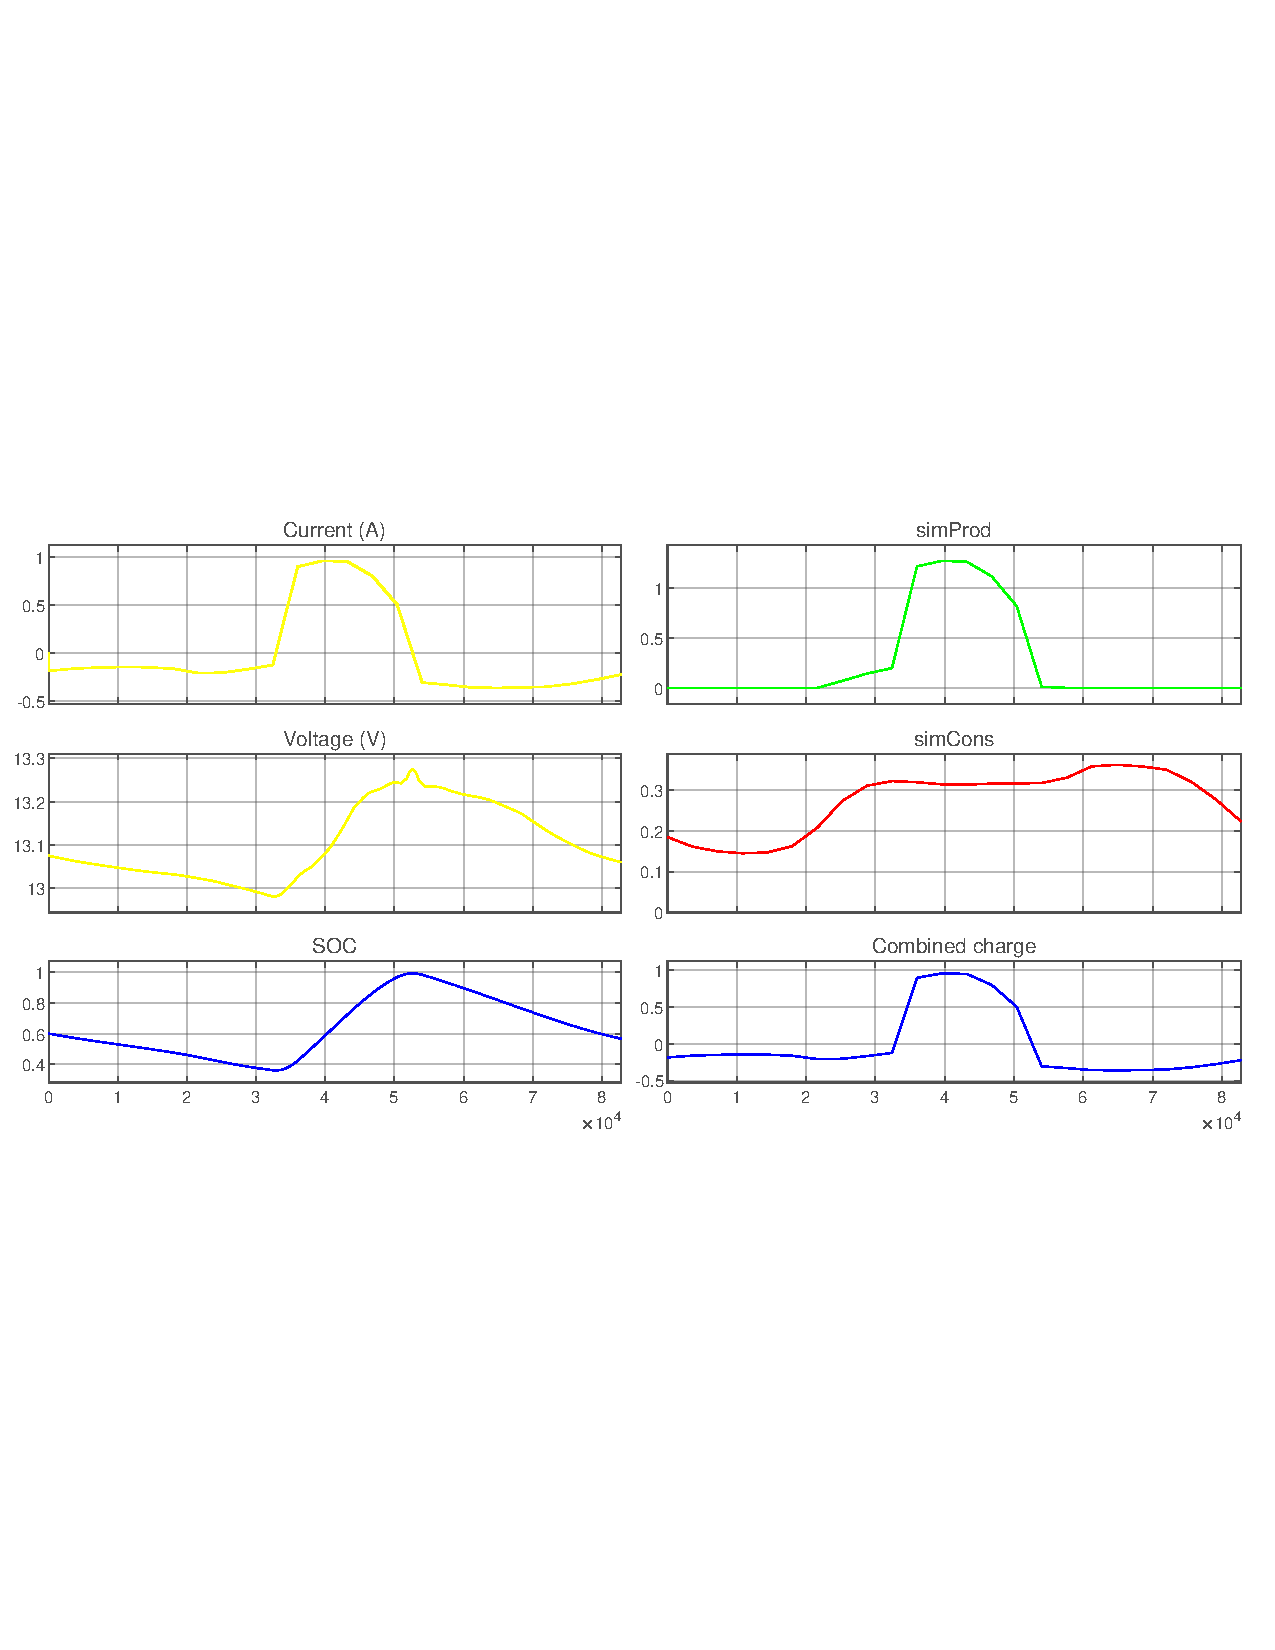
\includegraphics[width=\linewidth]{photos/Method_simulation.pdf}
    \caption{Simulation of how the daily consumption and production would be using an arbitrary value formatted from the national grid load in  figure \ref{method:fig:gridloadalbania}.}
    \label{method:fig:method_simulation}
\end{figure}
In this simulation, the SOC starts and ends at around the same value. Looking at the data from the results, this is an important factor of how well the system will do over time. If the SOC is higher after one 24-hour cycle, than the system is in surplus. If it is lower, than the system will eventually drain into empty. Production for this simulation is taken from January with a BH 800 system. As the graph shows an increase from 0.4 to 1 in SOC, that will not be enough to fully charge the system from empty. This is the factors we will look at in chapter \ref{ch:results}.

To analyze the daily load profile, we asked the questions of how long they are on, what power setting, and when they are on. We asked the same questions for charging from the USB-A port, besides power setting. No data was gathered on how many lamps are on, and if it is Fixed-Focus or Tube light. As we saw from the scenario consumption table \ref{table:power_configurations_all_systems}, this varies a lot for each configuration. Data for this needs to be estimated to create a daily load profile, based on observations and conversation in interviews. 

\subsection{Confidence intervals}
With a small set of data points, the \acrfull{ci} explains the uncertainty we are dealing with. \citep{lovasStatistikkUniversiteterOg2018} refers to student-t distribution when the sample size is below 30. We can apply confidence intervals for the consumption data gathered from the interviews. For consumption data we compare the hourly data points for each of the systems. Creating a point estimator for the standard deviation($s$) and the mean($\bar{x}$). These data will give us the indication of the uncertainty of the data. The reason to not do this with production data, is that the data points are an estimation. As the data is simulated from one setup, there is no variation in the output. Although we could create a CI based on the weather irregularities, this would be inaccurate as the irradiance mean will change throughout the month. 
\section{Economic metrics}

\subsection{Electricity price}
%Explain where the price was found had how we can forecast the price further
The Albanian Power Exchange has dataset of the spot price during 2024 we can use in our calculations\citep{albanianpowerexchangeDAMAlbania20242025}. In addition, we will ask questions of how much a person pays in electricity bills each month to get a rough estimate if that spot price applies for them. From the 2024 report of the Albanian Power Exchange, we get that the mean spot price was 0.112€/KWh. This was an 11,84\% increase from 2023. The report also showed how Albania is importing large amounts of power from Kosovo, being in production deficit themselves. As this power exchange started in 2023, we have no more historical data of the electricity price from this source. 

In figure \ref{method:fig:EU27_elecprice}, we can see how the Albanian electricity price compares to the average for EU-27. The data of the price is in \acrfull{euro}, although Albanians pay in \acrfull{lek}. 

\begin{figure}[H]
    \centering
    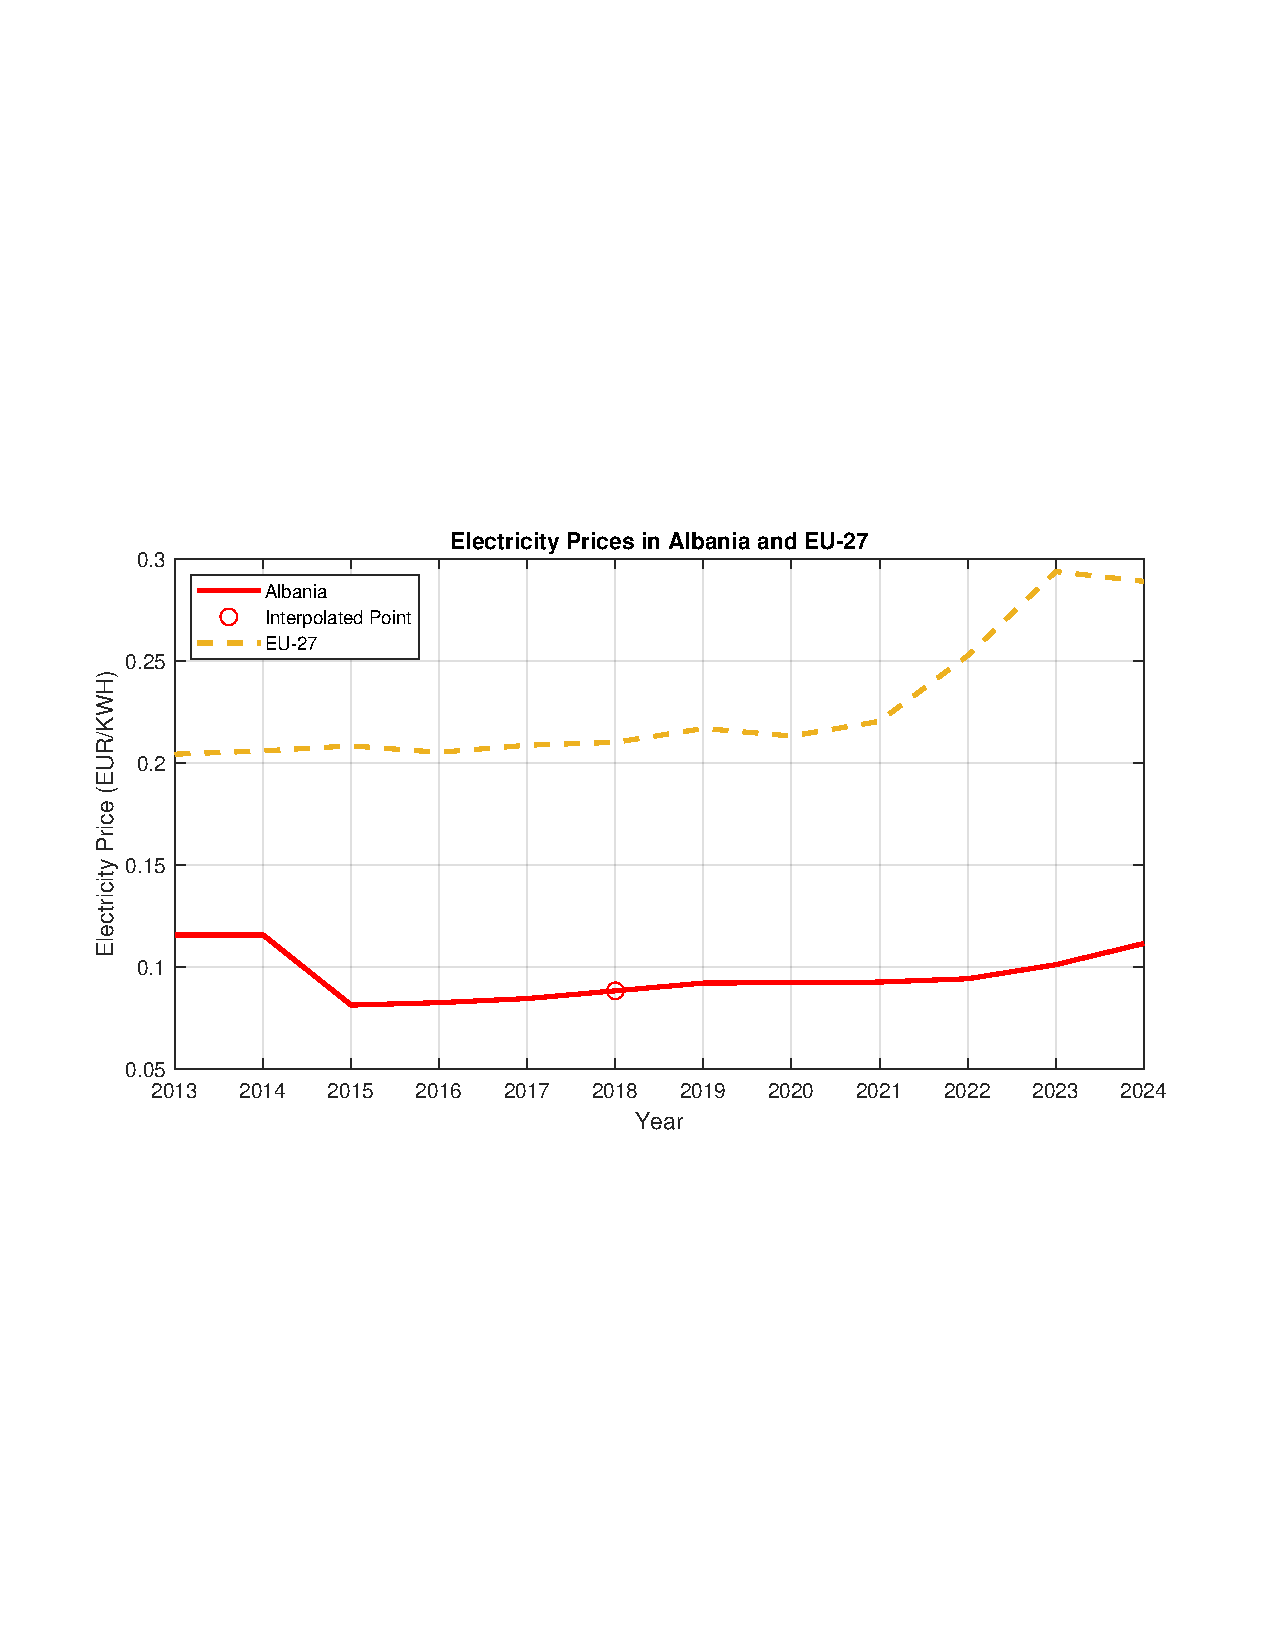
\includegraphics[width=\linewidth]{photos/EU27Electricity_Prices.pdf}
    \caption{One interpolated point due to lack of data in 2018. Data is for a medium size household\citep{eurostatElectricityPricesType2022}}
    \label{method:fig:EU27_elecprice}
\end{figure}

The electricity price for Albanians have been lower than EU-27, but has had a significant rise in the latest years.


Albania charges a fixed price for their electricity per kWh to households, not the spot price they pay for imports. This price will be decreased for household using below \SI{700}{\kilo\watt\hour} per month from 9,5 \acrshort{lek} to 8,5 \acrshort{lek}\citep{euronewsalbaniaImplementationNewElectricity2025}. The price increase in figure \ref{method:fig:EU27_elecprice} is due to the currencies changing in value. Due to the price being relatively stable, and the life cycle being only 7 years, we will not create an electricity forecast for the price. 

\subsection{SHS cost}
Participants of the project was given their system for free. This means that there are two different points of view to take for analysis of the cost of the systems. Either lifetime costs without the investment cost, or lifetime costs with investment cost. Although the product is not sold by Bright Products on the commercial market, third-party retailers sell the product. 

\begin{table}[h]
\centering
\begin{tabularx}{\textwidth}{|X|X|X|}
\hline
\textbf{System} & \textbf{Third-party retail price[EUR]} & \textbf{Bright quantity price[USD]} \\ \hline
BH 300        &  275 & 124 \\ \hline
BH 600        &  367 & 160 \\ \hline
BH 800        &  468 & 222 \\ \hline
\end{tabularx}
\caption{Light module inventory of systems. \textit{Min [lm]} is when all lights on low power setting, \textit{Max [lm]} is when all lights are on full power setting.}
\label{table:SHS_cost}
\end{table}

The lifetime of this system is given in 6-7 years or 2000 charge cycles\footnote{A charge cycle of the battery is defined as it discharging from full to empty, and back up to full.}. There is no more maintenance required to fulfill the given lifetime. Apart from possible malfunction and replacement of the malfunctioning parts, there are no planned costs of owning the SHS.

We also included the question of \textit{What would be a fair price for this system?} in our field trip questions \ref{apx:ftquestions}. The intention of this question was to reveal what the product would have to be priced at for the participants to buy this. Answering if the participants would be able to afford this system at all, or at least how much each participant would be able to share the cost of the system.

\subsection{Levelized Cost of Energy}
\label{chap:method:sec:LCOE}
To evaluate the \acrshort{lcoe}, we will take the cost of buying the product from either Third-party or in quantity from Bright. Lifetime is assumed to be either 2000 charge cycles or 6 to 7 years. As $\frac{2000}{365.25} \approx 5.5$, the lifetime will be based on cycles if the system does one charge cycle each day continuously throughout it's lifetime. Solar panels are expected to last 25-30 years, although \citep{sodhiEconomicLifetimesSolar2022} claims that their realistic lifetime will be shorter based on reduced efficiency. Battery is the bottleneck that Bright refers to for the lifetime of the system. \citep{pregerDegradationCommercialLithiumIon2020} found that \acrfull{lfp} can last up to 9000 cycles before going to 80\% of initial capacity. FLP is the battery type in all of the systems from Bright.


Table \ref{table:cost_per_system} shows the cost of a system per year for the entire lifetime. The lifetime used is based on the minimum expected lifetime, given lifetime from specifications, and the maximum amount of lifetime for the battery. This is all given that the battery will complete a charge cycle each day throughout it's lifetime. 

\begin{table}[H]
\centering
\small
\begin{tabularx}{0.3\textwidth}{|>{\RaggedRight\hsize=0.4\hsize}X|>{\Centering\hsize=0.3\hsize}X|>{\Centering\hsize=0.3\hsize}X|}
\hline
\multicolumn{3}{|c|}{BH 300 System} \\
\hline
\textbf{$C/L$} & \textbf{$C_R$} & \textbf{$C_Q$} \\
\hline
\textbf{$L_{min}$} & 50.2 & 22.6 \\ \hline
\textbf{$L_{6}$} & 45.8 & 20.7 \\ \hline
\textbf{$L_{7}$} & 39.3 & 17.7 \\ \hline
\textbf{$L_{max}$} & 11.2 & 5.0 \\ \hline
\end{tabularx}%
\hspace{0.5em}% Litt horisontal avstand mellom tabellene
\begin{tabularx}{0.3\textwidth}{|>{\RaggedRight\hsize=0.4\hsize}X|>{\Centering\hsize=0.3\hsize}X|>{\Centering\hsize=0.3\hsize}X|}
\hline
\multicolumn{3}{|c|}{BH 600 System} \\
\hline
\textbf{$C/L$} & \textbf{$C_R$} & \textbf{$C_Q$} \\
\hline
\textbf{$L_{min}$} & 67.0 & 29.2 \\ \hline
\textbf{$L_{6}$} & 61.2 & 26.7 \\ \hline
\textbf{$L_{7}$} & 52.4 & 22.9 \\ \hline
\textbf{$L_{max}$} & 14.9 & 6.5 \\ \hline
\end{tabularx}%
\hspace{0.5em}% Litt horisontal avstand mellom tabellene
\begin{tabularx}{0.3\textwidth}{|>{\RaggedRight\hsize=0.4\hsize}X|>{\Centering\hsize=0.3\hsize}X|>{\Centering\hsize=0.3\hsize}X|}
\hline
\multicolumn{3}{|c|}{BH 800 System} \\
\hline
\textbf{$C/L$} & \textbf{$C_R$} & \textbf{$C_Q$} \\
\hline
\textbf{$L_{min}$} & 85.5 & 40.5 \\ \hline
\textbf{$L_{6}$} & 78.0 & 37.0 \\ \hline
\textbf{$L_{7}$} & 66.9 & 31.7 \\ \hline
\textbf{$L_{max}$} & 19.0 & 9.0 \\ \hline
\end{tabularx}
\caption{Cost per year for each system in EUR. Where $L_{min}$ is 2000 charge cycles, $L_{6}$, $L_{7}$ is 6 and 7 years, and $L_{max}$ is 9000 charge cycles. $C_R$ is the retail price, and $C_Q$ is the discounted quantity price.}
\label{table:cost_per_system}
\end{table}

Maintenance costs for the system is not included, but would be expected on a system that has 9000 cycles. Table \ref{table:cost_per_system} also shows how much the system needs to yield each year to be profitable. Comparing this to the amount of electricity produced and consumed from the system, we can see if this system would be a worthwhile investment. If the usage is low on all systems, smaller systems can be more profitable. A BH 300 system only needs to cover €5 of reduced electricity costs a year to be profitable if doing 9000 cycles. 

\subsection{Discount rate}
Using equation \eqref{eq:ramseyformula}, we can find the SDR in equation \eqref{eq:socialdiscountrate}. \citep{internationalmonetaryfundALBANIA2024ARTICLE2025} estimate the long-term real \acrfull{gdp} growth of Albania to about 3.5\%. The pure time preference is set to 0, as we don't have any data on this. $\eta$ is set to 1.5 as the SHS targets low-income households, where increasing consumption is prioritized. 

\begin{align}
    r & =  0 + 1.5\cdot3.5 = \textbf{5.25\%}
    \label{eq:socialdiscountrate}
\end{align}

\citep{inproceedings} used the discount rate of 7\% for a wind farm project in Albania. Being a renewable energy project, it is similar to "Use the Sun". It differs as SHS is a targeted measure towards low-income households, and is primarily humanitarian aid.
\subsection{Payback time}
Using data from table \ref{table:SHS_cost} and the income, we can find the payback time for a system. With data from the question \textit{What do you think a fair price for this product would be if you were to buy it now?} we can compare the actual payback time with what the participants would accept as a payback time. \citep{inproceedings} reported a 7.6 and 8 year payback time for a utility wind farm in Albania. \citep{mannesEnduserEvaluationSolar2017} reported a 44 year payback time for a SHS in South Africa. Theses numbers show that the normal payback time for a SHS is higher than can be expected from a normal investment. \citep{hoqueEvaluationEnergyPayback2014} uses energy yield as a payback indicator based on the CO2 emissions caused by production. They found that in Bangladesh it takes around 7 years for a SHS to produce enough to recover the emissions lost from production. They also assume a 20 year lifespan in the SHS. 

\section{Social}
To analyze the social effects of this project, we needed questions regarding the overall changes this system made to their life. This includes the way they interact with and use the system, how they maintain it, and how their view on solar power systems. Participant's financial situation were generally below average for the area, giving rise to another set of social metrics. How large the cost of electricity is compared to their budget will give a pointer of what impact this system has for them. Households will be of different amount of people, and the use of such a system will benefit more people if the home is more populated. 

\subsection{Power outages}
\label{ch:metod:powerout}
Although Albania has full grid coverage, as mentioned in chapter \ref{ch:intro} - power outages still occur. \citep{nduhuuraImpactsElectricityOutages2021} shows that areas that have full grid coverage still may not have reliable power transmission. The study looks at how power outages in Ghana had diverse outcomes for households, reducing security and increasing food spoilage. Although food spoiling will not be relevant for this small of a system, the increased security will. Asking questions about power outages and their effects will help us do an evaluation of the social benefits participants get. Candles are common as alternative lighting when there is power outages, being a cheap emergency solution. \citep{martyahrensHomeCandleFires2020} shows that in the US, 2\% of home fires and 6\% of home fire injuries are due to candles. Candles are mostly used from decoration in the US, meaning that the use and dangers may be higher in developing countries. 

\subsection{Technology adoption}
Solar power is an old technology, but has not been widely used until recent years. Introducing solar power requires some understanding of the use and functionality of the system. As mentioned in chapter \ref{ch:theory}, angle, azimuth and soling can have a large impact on the efficiency of the panel. As mentioned in chapter \ref{ch:background}, some studies claimed training as a barrier to entry. Although there is a manual with some easy setup steps for the system, getting an optimal use out of the system requires specific knowledge. As the caption from figure \ref{method:fig:wattage_generation_PV40wpp} reveals, the optimal values for this area are not the ones given as a general rule of thumb. An azimuth $\phi=35\degree$ is not the typical $0\degree$ given as standard for the northern hemisphere. As there are many functional tilt angles and azimuths for the panel, we will measure how well each of the different setups work. Comparing it towards the optimal, we can then see if there is a need for better installation training of the systems or if the manual was sufficient. 

\subsection{Solar energy awareness}
One of the project goals was to educate communities about the benefits of solar energy. Showing participants how using solar power can supply them directly with electricity and not supplied from the grid would hopefully encourage to more use of this power source. As mentioned in chapter \ref{ch:background}, Albania has solar ongoing solar energy projects that seek to increase the capacity. We asked the question of \textit{What are your thoughts on solar power as an energy resource?}, intending to get an answer of how receiving the solar panel has affected their thoughts. 

